%
% This is a borrowed LaTeX template file for lecture notes for CS267,
% Applications of Parallel Computing, UCBerkeley EECS Department.
% Now being used for CMU's 10725 Fall 2012 Optimization course
% taught by Geoff Gordon and Ryan Tibshirani.  When preparing 
% LaTeX notes for this class, please use this template.
%
% To familiarize yourself with this template, the body contains
% some examples of its use.  Look them over.  Then you can
% run LaTeX on this file.  After you have LaTeXed this file then
% you can look over the result either by printing it out with
% dvips or using xdvi. "pdflatex template.tex" should also work.
%

\documentclass[twoside]{article}
\setlength{\oddsidemargin}{0.25 in}
\setlength{\evensidemargin}{-0.25 in}
\setlength{\topmargin}{-0.6 in}
\setlength{\textwidth}{6.5 in}
\setlength{\textheight}{8.5 in}
\setlength{\headsep}{0.75 in}
\setlength{\parindent}{0 in}
\setlength{\parskip}{0.1 in}

%
% ADD PACKAGES here:
%

\usepackage{amsmath,amsfonts,graphicx}

%
% The following commands set up the lecnum (lecture number)
% counter and make various numbering schemes work relative
% to the lecture number.
%
\newcounter{lecnum}
\renewcommand{\thepage}{\thelecnum-\arabic{page}}
\renewcommand{\thesection}{\thelecnum.\arabic{section}}
\renewcommand{\theequation}{\thelecnum.\arabic{equation}}
\renewcommand{\thefigure}{\thelecnum.\arabic{figure}}
\renewcommand{\thetable}{\thelecnum.\arabic{table}}

%
% The following macro is used to generate the header.
%
\newcommand{\lecture}[4]{
   \pagestyle{myheadings}
   \thispagestyle{plain}
   \newpage
   \setcounter{lecnum}{#1}
   \setcounter{page}{1}
   \noindent
   \begin{center}
   \framebox{
      \vbox{\vspace{2mm}
    \hbox to 6.28in { {\bf EE402 - Discrete Time Systems
	\hfill Spring 2018} }
       \vspace{4mm}
       \hbox to 6.28in { {\Large \hfill Lecture #1 \hfill} }
       \vspace{2mm}
       \hbox to 6.28in { {\it Lecturer: #2 \hfill } }
      \vspace{2mm}}
   }
   \end{center}
   \markboth{Lecture #1}{Lecture #1}

   \vspace*{4mm}
}
%
% Convention for citations is authors' initials followed by the year.
% For example, to cite a paper by Leighton and Maggs you would type
% \cite{LM89}, and to cite a paper by Strassen you would type \cite{S69}.
% (To avoid bibliography problems, for now we redefine the \cite command.)
% Also commands that create a suitable format for the reference list.
\renewcommand{\cite}[1]{[#1]}
\def\beginrefs{\begin{list}%
        {[\arabic{equation}]}{\usecounter{equation}
         \setlength{\leftmargin}{2.0truecm}\setlength{\labelsep}{0.4truecm}%
         \setlength{\labelwidth}{1.6truecm}}}
\def\endrefs{\end{list}}
\def\bibentry#1{\item[\hbox{[#1]}]}

%Use this command for a figure; it puts a figure in wherever you want it.
%usage: \fig{NUMBER}{SPACE-IN-INCHES}{CAPTION}
\newcommand{\fig}[3]{
			\vspace{#2}
			\begin{center}
			Figure \thelecnum.#1:~#3
			\end{center}
	}
% Use these for theorems, lemmas, proofs, etc.
\newtheorem{theorem}{Theorem}[lecnum]
\newtheorem{lemma}[theorem]{Lemma}
\newtheorem{proposition}[theorem]{Proposition}
\newtheorem{claim}[theorem]{Claim}
\newtheorem{corollary}[theorem]{Corollary}
\newtheorem{definition}[theorem]{Definition}
\newenvironment{proof}{{\bf Proof:}}{\hfill\rule{2mm}{2mm}}

% **** IF YOU WANT TO DEFINE ADDITIONAL MACROS FOR YOURSELF, PUT THEM HERE:

\begin{document}

% Lecture Details
\lecture{9}{Asst. Prof. M. Mert Ankarali}
....

\section*{Steady-Sate (DC) Response Analysis}

Let's remember the final value theorem. Given a discrete time signal 
$x[k]$ and its z-transform $X(z)$, if $x[k]$ is convergent sequence
final value theorem states that
%
\begin{align*}
\lim_{k\to \infty} x[k] &= \lim_{z \to 1} \left[ \left( 1 - z^{-1} \right)
  X(z) \right]
\\
x_{ss} &= \lim_{z \to 1} \left[ \frac{z-1}{z} X(z) \right]
\end{align*}

    \begin{center}
\begin{minipage}[h]{0.99\linewidth}
    \begin{center}
      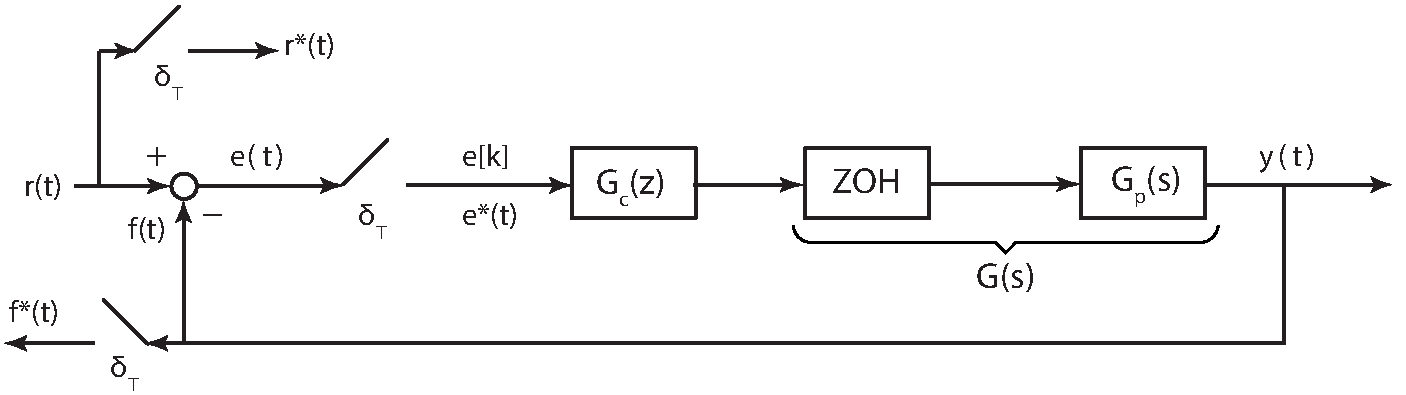
\includegraphics[width=\textwidth]{digitalblock}
    \end{center}
\end{minipage}
    \end{center}

Now let's find the pulse transfer function from the reference signal
$r[k]$ to the error signal $e[k]$, to further analyze the steady-state
error response. 
%
\begin{align*}
E(z) &= R(z) - E(z) \left( G_c(z) G(z) \right) , \quad \mathrm{where} \
  G(z) = \mathcal{Z} \lbrace G(s) \rbrace
\\
\frac{E(z)}{R(z)} &= \frac{1}{1 + G_c(z) G(z) }
\end{align*}
%
Note that $G_c(z) G(z)$ is the pulse transfer function from the error
signal $E(z)$ to the signal which is fed to the negative terminal of 
the main difference operator, i.e. $F(z)$. This transfer function is
called feed-forward or open-loop  pulse transfer function of the 
closed-loop digital control system. For this system, 
%
\begin{align*}
\frac{F(z)}{E(z)} = G_{OL} = G_c(z) G(z)
\end{align*}
%
Then $E(z)$ can be written as
%
\begin{align*}
E(z) = R(z) \frac{1}{1 + G_{OL} (z) }
\end{align*}
%
It is obvious that first requirement on m steady-state error
performance is that closed-loop system have to be stable.
Now let's analyze specific but fundamental input scenarios. 

\subsection*{Unit-Step Input}

We know that $r[k] = u[k]$ and $R(z) = \frac{1}{1 - z^-1}$ then 
we have
%
%
\begin{align*}
e_{ss} &= \lim_{z \to 1} \left[ \left(1 - z^{-1} \right) R(z) \frac{1}{1
         + G_{OL} (z) } \right]
\\
&= \lim_{z \to 1} \left[ \left(1 - z^{-1} \right) \frac{1}{1-z^{-1}} \frac{1}{1
         + G_{OL} (z) } \right]
\\
e_{ss} &= \frac{1}{1 + \lim_{z \to 1} G_{OL} (z) }
\end{align*}
%
If the DC gain of the system (also called static error constant) is
constant, i.e. $G_{OL}(1) = K_{DC}$ then the steady state error can be
computed as
%
\begin{align*}
e_{ss} &= \frac{1}{1 + K_{DC}}
\end{align*}
%
It is obvious that 
%
\begin{align*}
e_{ss} &\neq 0 \quad \mathrm{if} \quad |K_{DC}| < \infty
\\
e_{ss} &\to 0 \quad \mathrm{if} \quad K_{DC} \to \infty
\end{align*}
%
Based on these results, we can have the following conclusions
%
\begin{itemize}
\item If $G_{OL} (1) = 0$, then $e_{ss} = 1$. These are \textbf{type
  \textit{negative}} systems, and the steady-state error of step 
response type signals are always $100 \%$.
\item If $G_{OL} (1) = K_{DC}$ , $0 < | K_{DC} | < \infty$, then $e_{ss} =
  1/(1 + K_{DC})$. These are \textbf{type 0} systems. We observe a
  bounded steady-state error and it is possible to reduce the by increasing the static gain
constant $K_P$. 
\item  If $G_{OL} (1) = \infty$, then $e_{ss} = 0$. These are
  \textbf{type \textit{positive}} systems. The steady-state error
  is perfectly zero for such systems.
\end{itemize}

Now let's generalize the \textit{type} of systems. An \textit{N type}
closed loop system has the following form of open-loop pulse transfer 
function
%
\begin{align*}
G_{OL}(z) &= \frac{1}{(z-1)^N} G_{DC}(z) \\
| G_{DC}(1) | &= K_{DC} \quad \mathrm{where} \ 0 < | K_{DC} | < \infty
\end{align*}
% 
It is easy to see that for unit-step response
%
\begin{itemize}
\item Type $N < 0$: $e_{ss} = 1$ (or $e_{ss} =100 \%$)
\item Type $N = 0$: $e_{ss} =  1/(1 + K_{DC})$
\item Type $N > 0$: $e_{ss} = 0$
\end{itemize}

\subsection*{Unit-Ramp Input}
%
We know that $r[k] = k u[k]$ and $R(z) = \frac{z^{-1}}{(1 - z^{-1})^2}$ then
we have

\begin{align*}
e_{ss} &= \lim_{z \to 1} \left[ \left(1 - z^{-1} \right) R(z) \frac{1}{1
         + G_{OL} (z) } \right]
\\
&= \lim_{z \to 1} \left[ \left(1 - z^{-1} \right) 
  \frac{z^{-1}}{(1 - z^{-1})^2} \frac{1}{1 +\frac{1}{(z-1)^N} G_{DC}(z) } \right]
\\
&= \lim_{z \to 1} \left[ \frac{1}{z - 1} \frac{1}{1 +\frac{1}{(z-1)^N}
  G_{DC}(z) } \right]
\\
&= \lim_{z \to 1} \left[ \frac{1}{(z-1) +\frac{1}{(z-1)^{N-1}}
  G_{DC}(z) } \right]
\\
e_{ss} &=  \frac{1}{ \lim_{z \to 1} \left[ \frac{1}{(z-1)^{N-1}}
  G_{DC}(z) \right] }
\end{align*}
%
Based on this result we can have the following steady-state
error conditions for the unit-ramp input based on the type 
condition of the system
%
\begin{itemize}
\item Type $N < 1$: $e_{ss} \to  \infty$
\item Type $N = 1$: $e_{ss} = \frac{1}{K_{DC}}$
\item Type $N > 1$: $e_{ss} = 0$
\end{itemize}
%
\subsection*{Unit-Quadratic (Acceleration) Input}
%
We know that $r[k] = \frac{1}{2} k^2 u[k]$ and $R(z) = \frac{z^{-1} (1
  + z^{-1})}{2 (1 - z^{-1})^3}$ then
we have
\begin{align*}
e_{ss} &= \lim_{z \to 1} \left[ \left(1 - z^{-1} \right) R(z) \frac{1}{1
         + G_{OL} (z) } \right]
\\
&= \lim_{z \to 1} \left[ \left(1 - z^{-1} \right) 
 \frac{z^{-1} (1 + z^{-1})}{2 (1 - z^{-1})^3} 
  \frac{1}{1 +\frac{1}{(z-1)^N} G_{DC}(z) } \right]
\\
&= \lim_{z \to 1} \left[ \frac{(z+1)}{2 (z - 1)^2} \frac{1}{1 +\frac{1}{(z-1)^N}
  G_{DC}(z) } \right]
\\
&= \lim_{z \to 1} \left[ \frac{(z+1)/2}{(z-1)^2 +\frac{1}{(z-1)^{N-2}}
  G_{DC}(z) } \right]
\\
e_{ss} &=  \frac{1}{ \lim_{z \to 1} \left[ \frac{1}{(z-1)^{N-2}}
  G_{DC}(z) \right] }
\end{align*}
%
\begin{itemize}
\item Type $N < 2$: $e_{ss} \to  \infty$
\item Type $N = 2$: $e_{ss} = \frac{1}{K_{DC}}$
\item Type $N > 2$: $e_{ss} = 0$
\end{itemize}
%

\paragraph{Example 1:} $G(z) = \frac{z-1}{z-0.5}$ and $G_C(z) =
K$. Compute the steady-state erro to unit-step, unit-ramp, a
and unit-quadratic inputs.

\paragraph{Solution:} 
%
\begin{align*}
G_{OL}(z) &= K \frac{z-1}{z-0.5} = \frac{1}{(z-1)^{-1}} \frac{K}{z-0.5}
\\
G_{DC}(1) &= 2 K \quad, \mathrm{Type} \ -1 
\end{align*}
%
Then the steady-state errors are computed as
\begin{itemize}
\item Unit-step: $e_{ss} = 1$
\item Unit-ramp: $e_{ss} = \infty$
\item Unit-acceleration: $e_{ss} = \infty$
\end{itemize}

\paragraph{Example 2:} $G(z) = \frac{z-1}{z-0.5}$ and $G_C(z) =
K \frac{z}{z-1}$. Compute the steady-state error to unit-step, unit-ramp, a
and unit-quadratic inputs.

\paragraph{Solution:} 
%
\begin{align*}
G_{OL}(z) &= \frac{K z}{z-0.5} 
\\
G_{DC}(1) &= 2 K \quad, \mathrm{Type} \ 0 
\end{align*}
%
Then the steady-state errors are computed as
%
\begin{itemize}
\item Unit-step: $e_{ss} = \frac{1}{1 + 2 K}$
\item Unit-ramp: $e_{ss} = \infty$
\item Unit-acceleration: $e_{ss} = \infty$
\end{itemize}

\paragraph{Example 3:} $G(z) = \frac{z-1}{z-0.5}$ and $G_C(z) =
K \frac{z^2}{(z-1)^2}$. Compute the steady-state erro to unit-step, unit-ramp, a
and unit-quadratic inputs.

\paragraph{Solution:} 
%
\begin{align*}
G_{OL}(z) &= \frac{K z^2}{(z-1) (z-0.5)} = \frac{1}{z-1} \frac{K
            z^2}{z - 0.5}
\\
G_{DC}(1) &= 2 K \quad, \mathrm{Type} \ 1 
\end{align*}
%
Then the steady-state errors are computed as
%
\begin{itemize}
\item Unit-step: $e_{ss} = 0$
\item Unit-ramp: $e_{ss} = \frac{1}{2 K}$
\item Unit-acceleration: $e_{ss} = \infty$
\end{itemize}

\subsection*{Open-Loop Transfer Function for Different Topologies}

When computing the steady-state error it is important to 
carefully analyze the topology of the control system. 

Compute the $G_{OL}(z)$ for the following system

\begin{center}
\begin{minipage}[h]{0.6\linewidth}
    \begin{center}
      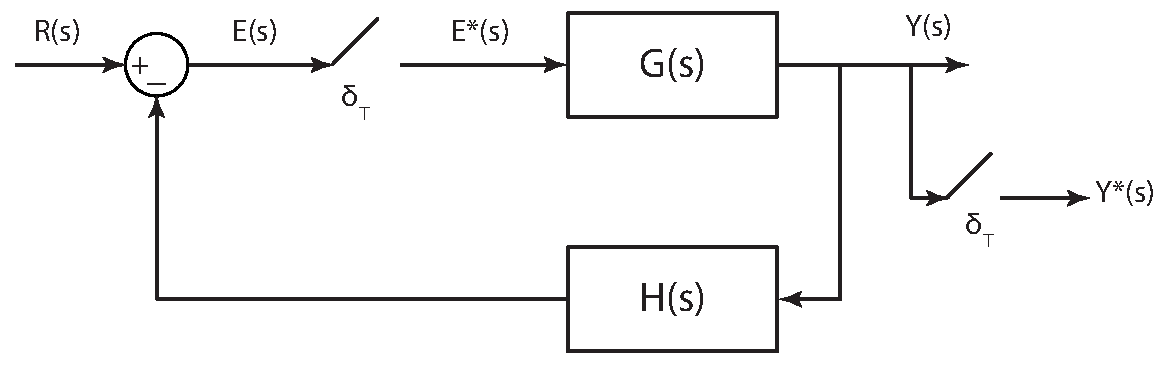
\includegraphics[width=\textwidth]{closed}
    \end{center}
\end{minipage}
\end{center}

\begin{align*}
F(s) &= E^*(s) G(s) H(s)
\\
F^*(s) &= E^*(s) [ G(s)H(s) ]^* = E^*(s) GH^*(s)
\\
G_{OL}(z) &= GH(z)
\end{align*}

Now let's compte the $G_{OL}(z)$ for the following system

\begin{center}
\begin{minipage}[h]{0.6\linewidth}
    \begin{center}
      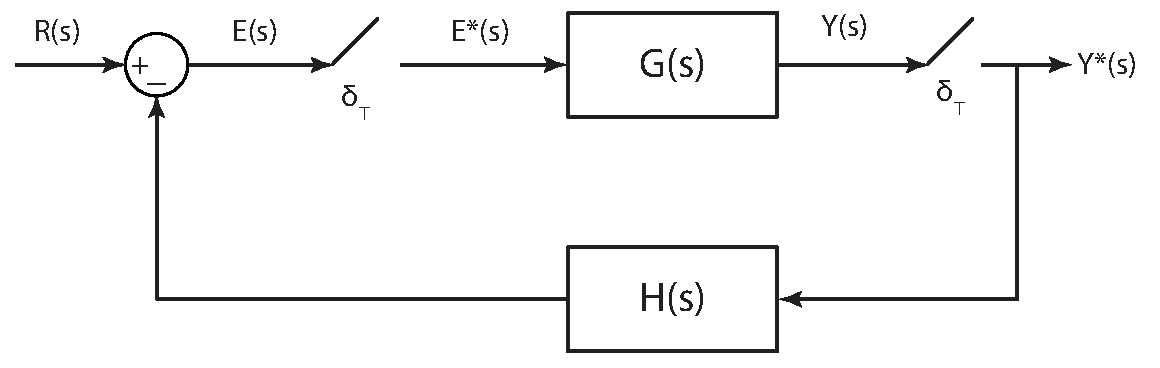
\includegraphics[width=\textwidth]{closed2}
    \end{center}
\end{minipage}
\end{center}

\begin{align*}
F(s) &= [ E^*(s) G(s) ]* H(s) = E^*(s) G^*(s) H(s) 
\\
F^*(s) &= E^*(s) G^*(s) H^*(s)
\\
G_{OL}(z) &= G(z) H(z)
\end{align*}

Now let's compte the $G_{OL}(z)$ for the following system

\begin{center}
\begin{minipage}[h]{\linewidth}
    \begin{center}
      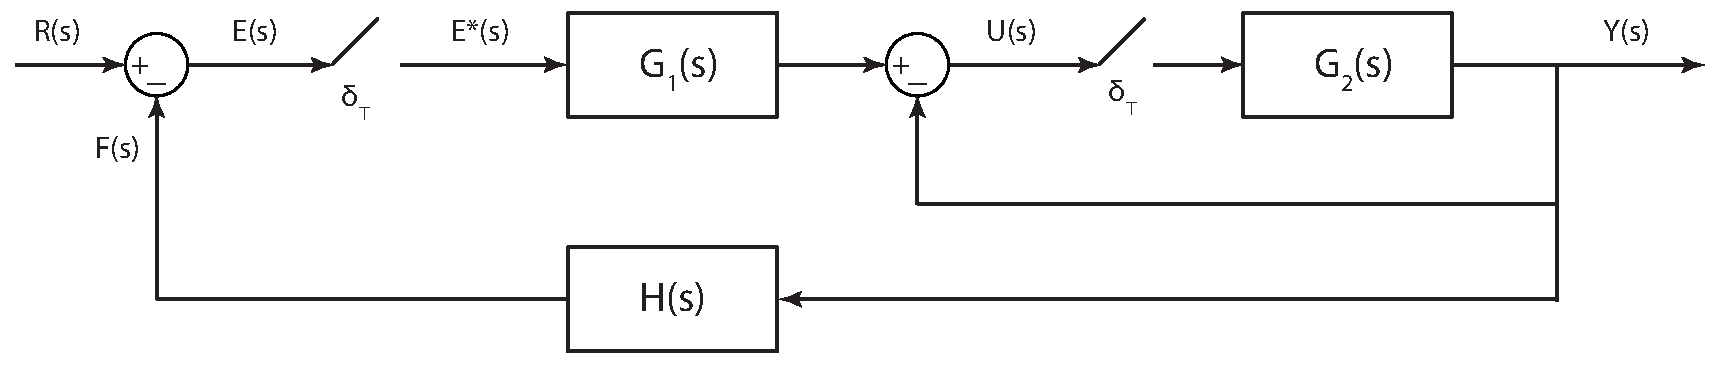
\includegraphics[width=\textwidth]{closed3}
    \end{center}
\end{minipage}
\end{center}

From last week we know that
%
\begin{align*}
U^*(s) = \frac{G_1^*(s)}{1 + G_2^*(s) + G_1^*(s) G_2 H^*(s)} R^*(s)
\end{align*}
%
Then we can 
%
\begin{align*}
U(s) = E^*(s) G_1(s) - U^*(s) G_2(s) \quad &\rightarrow \quad U^*(s) =
       E^*(s) G_1^*(s) - U^*(s) G^*_2(s)
\\
U^*(s) &= \frac{G_1^*(s)}{1 + G^*_2(s)} E^*(s)
\\
E^*(s) &= \frac{1 + G_2^*(s)}{1 + G_2^*(s) + G_1^*(s) G_2 H^*(s)} R^*(s)
\\
\frac{E(z)}{R(z)} &= \frac{1 + G_2(z)}{1 + G_2(z) + G_1(z) G_2 H(z)} 
\end{align*}
%
This transfer function form does not (directly) fit to the form we analyzed,
i.e. $\frac{E(z)}{R(z)} = \frac{1}{1 + G_{OL}(z) }$, so we can not
directly used the conditions and formulaes for this form. One way of
comuting the steady-state errors is directly applying the final-value theorem.

The other way is we can simply convert the computed pulse transer
function $E(z) / R(z)$ such that it fits the form $\frac{E(z)}{R(z)} = \frac{1}{1 + G_{OL}(z) }$.
If we carefully analyze the transer function we can obtain
%
\begin{align*}
\frac{E(z)}{R(z)} &= \frac{1}{1 + \frac{G_1(z) G_2H(z)}{1 + G_2(z)}} 
\\
G_{OL}(z) &= \frac{G_1(z) G_2H(z)}{1 + G_2(z)}
\end{align*}
%
It is also possible to derive $G_{OL}(z)$ via direct computation 
of $F(z) / E(z)$. 

\section*{Response to Disturbances}

When analyzing response of a system in addition to
the desired response to the reference input, it is also important
to analyze the response (both steady-state, transient, and frequency)
to unwanted disturbances and noises. 

\subsection*{Process Disturbance/Uncertainty/Noise}

Let's analyze a type of important disturbance on the fundamental 
discrete-time block diagram topology. 

\begin{center}
\begin{minipage}[h]{\linewidth}
    \begin{center}
      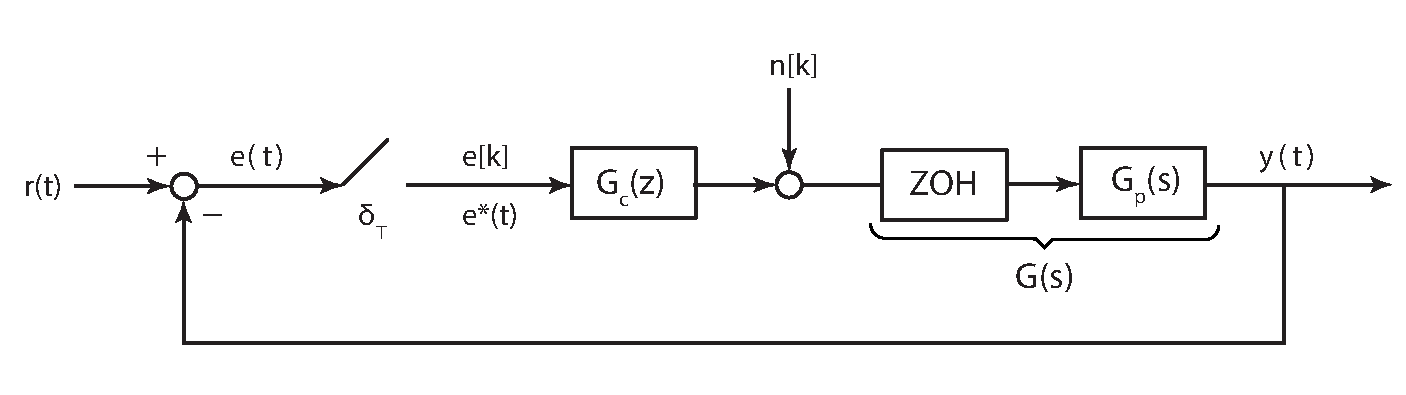
\includegraphics[width=\textwidth]{disturb}
    \end{center}
\end{minipage}
\end{center}

In order to analyze the response to the disturbance $n[k]$, we assume 
$r[k] = 0$ (which is just fine due to the linearity). Let's first find
the pulse transfer function from $N(z)$ to $Y(z)$. 

\begin{align*}
Y(z) &= ( -Y(z) G_c(z) + N(z) ) G(z)
\\
\frac{Y(z)}{N(z)} &= \frac{G(z)}{1 + G_c(z) G(z)}
\end{align*}

Technically, we want $\frac{Y(z)}{N(z)} = 0$, while also tracking
the reference signal. Since it is not perfectly possible to 
achieve $\frac{Y(z)}{N(z)} = 0$ while satisfying other constraints,
we want $\frac{Y(z)}{N(z)}$ to be ``small''. If $|G_C(z) G(z)| \gg 1$
then we have 

\begin{align*}
\frac{Y(z)}{N(z)} \approx \frac{1}{G_c(z)}
\end{align*}

Now let's consider a specific type of disturbance. An important
class of process disturbance/uncertainty is in the form of DC 
bias, i.e. $n(t) = N u(t)$ and $N(z) = \frac{N}{1 - z^{-1}}$. Let's
analyze DC steady state response using final value theorem.

\begin{align*}
y_{ss} &= \lim_{z\to1} \left[ \left( 1 - z^{-1} \right) Y(z) \right]
= \lim_{z\to1} \left[ \left( 1 - z^{-1} \right) N(z) \frac{G(z)}{1 +
  G_c(z) G(z)} \right]
\\
&= \lim_{z\to1} \left[ \left( 1 - z^{-1} \right) \frac{N}{1 - z^{-1}} \frac{G(z)}{1 +
  G_c(z) G(z)} \right]
= \lim_{z\to1} \left[ N \frac{G(z)}{1 +
  G_c(z) G(z)} \right]
\\
&= N \frac{\lim_{z\to1} G(z)}{1 + \lim_{z\to1} G_C(z) G(z) }
\end{align*}

Let's analyze the steady-state disturbance response

\begin{itemize}

  \item If plant is a type $< 0$ system (high pass filter plant)
    then $G(1) = 0$ and $y_{ss} = 0$. 

   \item If plant is a type $0$ system, then
%
\begin{align*}
y_{ss} &= \frac{N G(1)}{1 + G(1) \lim_{z\to1} G_C(z) }
\end{align*}
%
Now let's analyze the response based on the type of $G_c(z)$

\begin{itemize}

\item Type $< 0$, then 
%
\begin{align*}
y_{ss} &= N G(1)
\end{align*}
%
In this case, controller has no control
on the steady-state disturbance rejection
performance. 

\item Type $0$, then 
%
\begin{align*}
y_{ss} &= \frac{N G(1)}{1 + G(1) G_C(1) }
\end{align*}
%
Obviously in order to ``filter'' the disturbance 
we should select a $G_C(z)$ such that 
$| G_C(1) G(1) | \gg 1$ then
%
\begin{align*}
y_{ss} &= \frac{N}{G_C(1)}
\end{align*}
%
Large gain $G_C(z)$ can effectively filter the disturbance (but not completely). 

\item Type $> 0$, then 
%
\begin{align*}
y_{ss} &= \frac{N G(1)}{1 + G(1) \lim_{z\to1} G_C(z) }
\\
&= 0
\end{align*}
%
Integral action on $G_C(z)$ can perfectly 
reject the DC disturbance on steady state. 

\end{itemize}

\item If plant is a type $m > 0 $ then
%
\begin{align*}
y_{ss} &= \frac{N \lim_{z\to1} G(z)}{1 + \lim_{z\to1} G(z) G_C(z) } 
\\
\lim_{z\to1} G(z) &= \infty
\end{align*}
%
Depending on the type of $G_C(z)$, we can conclude that
%
\begin{itemize}
 \item Type $< 0$, $y_{ss} = \infty$
 \item Type $0$, $y_{ss} = C$, where $0 < C < \infty$
 \item Type $> 0$, $y_{ss} = 0$
\end{itemize}
%

\end{itemize}

\paragraph{Example 4:} $G(z) = \frac{z-1}{z-0.5}$ and $G_C(z) =
K$. Compute the steady-state response to a unit step
process disturbance/noise.

\paragraph{Solution:} 
%
\begin{align*}
y_{ss} = \frac{\lim_{z\to1}  \frac{z-1}{z-0.5}}{1 + \lim_{z\to1} K
  \frac{z-1}{z-0.5}} = 0
\end{align*}
%
Plant perfectly rejects disturbance. 
%

\paragraph{Example 5:} $G(z) = \frac{z}{z-0.5}$ and $G_C(z) =
K$. Compute the steady-state response to a unit step
process disturbance/noise.

\paragraph{Solution:} 
%
\begin{align*}
y_{ss} = \frac{\lim_{z\to1}  \frac{z}{z-0.5}}{1 + \lim_{z\to1} K
  \frac{z}{z-0.5}} = \frac{2}{1 + 2 K} 
\end{align*}
%
Large gain $K$ can be effective solution to reject disturbance
%

\paragraph{Example 6:} $G(z) = \frac{z}{z-0.5}$ and $G_C(z) = K_P +
K_I \frac{z}{z-1}$. Compute the steady-state response to a unit step
process disturbance/noise.

\paragraph{Solution:} 
%
\begin{align*}
y_{ss} = \frac{2}{1 + \lim_{z\to1} 2 \left(K_P + K_I  \frac{z}{z-1} \right)} = 0
\end{align*}
%
A PI controller can perfectly reject the DC process
disturbance. 
%

\subsection*{Measurement Disturbance/Uncertainty/Noise}

Let's analyze a different type of important disturbance on the fundamental 
discrete-time block diagram topology. 

\begin{center}
\begin{minipage}[h]{\linewidth}
    \begin{center}
      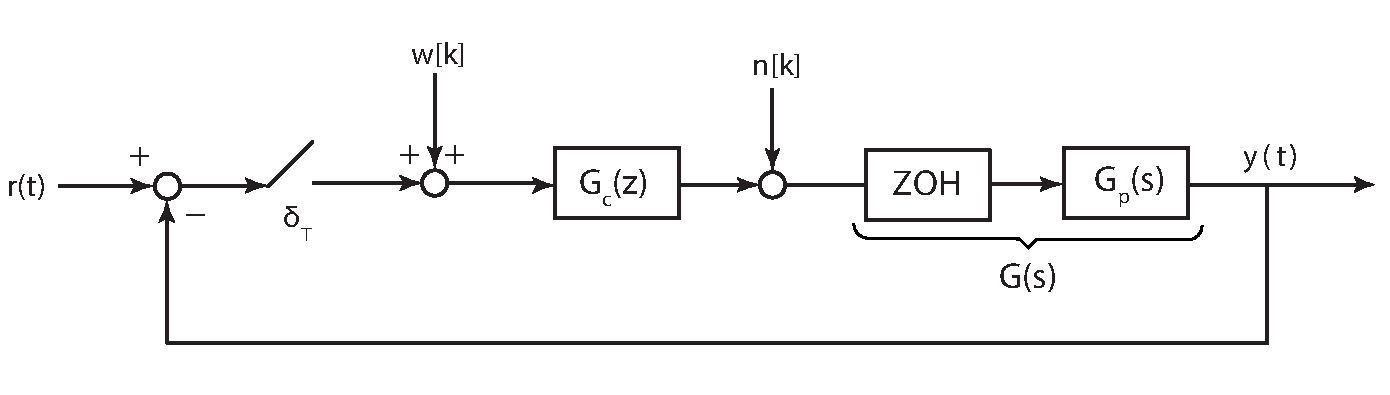
\includegraphics[width=\textwidth]{noise}
    \end{center}
\end{minipage}
\end{center}

In order to analyze the response to the disturbance $w[k]$, we assume 
$r[k] = 0$ and $n[k] = 0$ 

\begin{align*}
Y(z) &= ( W(z) -Y(z) ) G_c(z) G(z)
\\
\frac{Y(z)}{W(z)} &= \frac{G(z) G_C(z)}{1 + G_c(z) G(z)}
\\
&= \frac{G_{OL} (z)}{1 + G_{OL}(z)}
\end{align*}

Technically, we want $\frac{Y(z)}{N(z)} = 0$, while also tracking
the reference signal. Thus, practically we should design $G_C(z)$ such
that $|G_C(z) G(z)| \ll 1$, to eliminate measurement
noises/disturbances. (??????) 

\begin{align*}
\frac{Y(z)}{N(z)} \approx {G_{OL}(z)}
\end{align*}

This ``requirement'' obviously contradicts with 
requirements on stead-state tracking error performance
and process noise/disturbance rejection performance. Most well
known limitation of feedback control systems.

Now let's consider a specific type of measurement noise, i.e. DC measurement bias.  
$w(t) = W u(t)$ and $W(z) = \frac{W}{1 - z^{-1}}$. Let's
analyze DC steady state response using final value theorem.
%
\begin{align*}
y_{ss} &= \lim_{z\to1} \left[ (1 - z^{-1}) R(z) \frac{ G_{OL}(z) } {
  1 + G_{OL}(z) } \right] = \lim_{z\to1} \left[ (1 - z^{-1}) \frac{W}{1-z^{-1}} \frac{ G_{OL}(z) } {
  1 + G_{OL}(z) } \right]  
\\
&= \lim_{z\to1} \left[ \frac{ W G_{OL}(z) }{1 + G_{OL}(z) } \right]  
\end{align*}

Using the form $G_{OL}(z) = \frac{1}{(z-1)^N} G_{DC}(z)$, $y_{ss}$
takes the form
%
\begin{align*}
  y_{ss} &= \lim_{z\to1} \left[ \frac{ W G_{DC}(1) \frac{1}{(z-1)^N}} {1 + G_{DC}(1) \frac{1}{(z-1)^N}}\right]  
\end{align*}
%
Based on the type of the open-loop transfer function, $G_{OL}(z)$,
we can conclude 
%
\begin{itemize}
 \item Type $N < 0$: $y_{ss} = 0$. Perfect rejection of measurement
   bias, but we know that this is unacceptable from reference tracking
   point of view.
 \item Type $N = 0$
%
\begin{align*}
  y_{ss} &= \frac{ W G_{DC}(1) } {1 + G_{DC}(1) } 
\end{align*}
%
It seems that in order to ``filter'' the measurement bias
$G_{DC}(1)$ should be selected very small.

\item Type $N > 0$
%
\begin{align*}
  y_{ss} &= W 
\end{align*}
%
The disturbance is directly transfered to the output. 

\end{itemize}
% 


\paragraph{Example 7:} $G(z) = \frac{z-1}{z-0.5}$ and $G_C(z) =
K$. Compute the steady-state response to a unit step
measurement disturbance/noise.

\paragraph{Solution:} 
%
\begin{align*}
G_{OL}(z) &= K \frac{z-1}{z-0.5} \quad \textrm{Type} \ -1
\\
y_{ss} &= 0
\end{align*}
%
Plant perfectly rejects measurement bias. 
%

\paragraph{Example 8:} $G(z) = \frac{z}{z-0.5}$ and $G_C(z) =
K$. Compute the steady-state response to a unit step
process disturbance/noise.

\paragraph{Solution:} 
%
\begin{align*}
G_{OL}(z) &= K \frac{z}{z-0.5} \quad \textrm{Type} \ 0
\\
y_{ss} &= \frac{ 2K  } {1 +2K } 
\end{align*}
%
Small gain $K$ can be effective solution to reject measurement bias.
%

% **** This ENDS THE EXAMPLES. DON'T DELETE THE FOLLOWING LINE:
\end{document}